\section{SIM TIPS Simulator}

TIPS (Tips Is a Pixel Simulator) is mainly written in Python, but its core is based on aXeSIM, which is written in C and then wrapped in python by TIPS itself. The TIPS official gitlab repository can be found at the link

\begin{center}
\url{https://gitlab.euclid-sgs.uk/PF-SIM/SIM_TIPS_Simulator}    
\end{center}

Essentially TIPS has three main programs:

\begin{itemize}
\item \verb+EuclidNisSplit.py+: it creates the TIPS fits configuration and catalog files;
\item \verb+EuclidNisDetector.py+: it performs the pixel simulation at the single detector level, taking the configuration and catalog files as inputs;
\item \verb+EuclidNisCombine.py+: it takes all the 16 detector simulated frames and combines them into a single fits file.
\end{itemize}

\begin{figure}
    \centering
    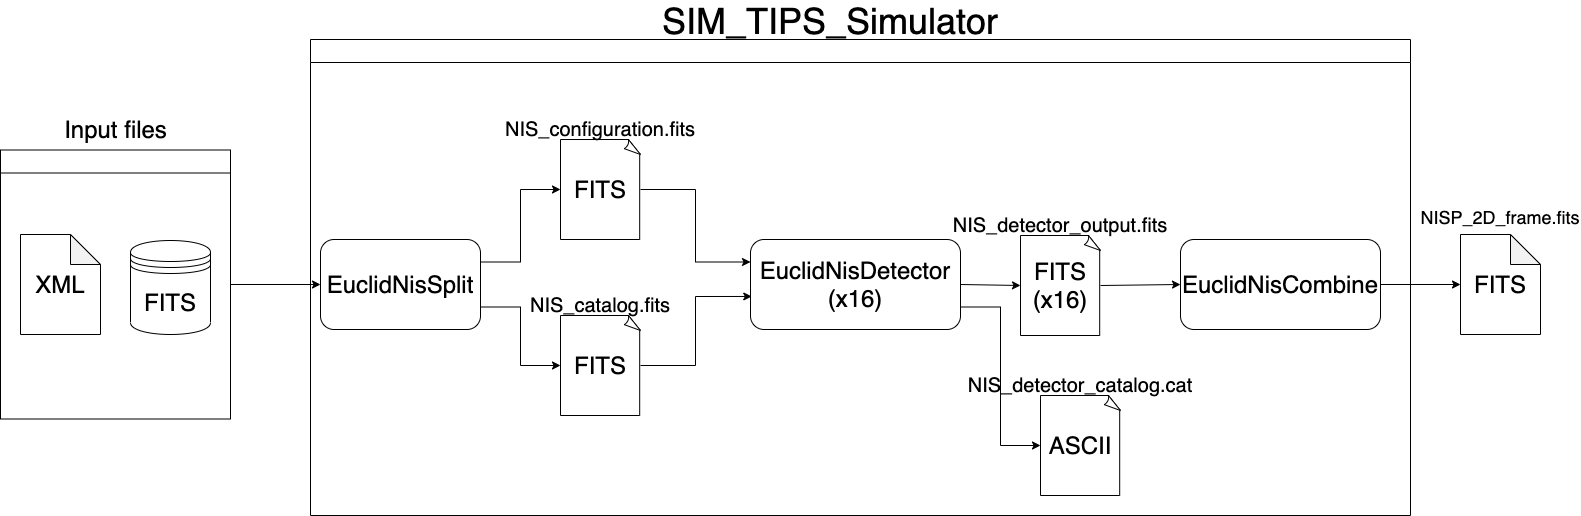
\includegraphics[scale=0.25]{figures/TIPS_workflow.png}
    \caption{Schematic representation of the workflow of TIPS.}
    \label{fig:TIPS_workflow}
\end{figure}

In the next section we describe the necessary input files for a TIPS simulation.

\subsection{TIPS input files}
In plain words, what TIPS needs to run a simulation can be summarized as follows:

\begin{itemize}
\item The catalogs of the sources (stars and galaxies) whose 2D spectra are to be simulated, optionally along with their spectra
\item The instrument and telescope configurations: i.e. the active instrumental effects, the grism used, the pointing coordinates, etc \dots
\item The Euclid Mission configuration, i.e. the Mission Database (MDB).
\end{itemize}

As shown in \figref{fig:TIPS_workflow} the input files needed for TIPS are essentially XML and FITS files. In particular, the input files passed explicitly as parameters to TIPS programs are XML files, some of them referencing the other input FITS files. Some useful links where to retrieve Euclid input files are

\begin{itemize}
\item Euclid Archive System (EAS): \url{https://eas-dps-cus.euclid.astro.rug.nl/}
\item Euclid Mission DataBase Viewer: \url{http://euclid.esac.esa.int/epdb/}
\end{itemize}

In what follows we give the details of our knowledge about the essential input files.

\subsubsection{XML input files}
Each of these files is a so-called \emph{DataProduct} (Dpd), i.e. a file which must have a precise format, maintained along with a specific software library (its Bindings) of classes to be read and written properly. In fact Data Products are the way with which the often the various Euclid Processing Functions (PFs) and Organization Units (OUs) exchange data. For example a specific DataProduct can be the output of one OU and the input for the next, or a common input for many OUs. Hence there must be a unique way to read and write the data contained in this file, in order to prevent possible compatibility problems.\\
In what follows we give a brief description of all the input XML data products needed by TIPS.

\paragraph{DpdNisInputConfiguration} 
The instrument and telescope configuration. It controls:

\begin{itemize}
\item The instrumental effects to be simulated, as boolean switches;
\item The spectral orders to be simulated, as capital letters. In particular letter A stands for 1st order, while subsequent letters characterize next orders. B means 0th order, C 2nd order and so on.
\item The telescope pointing coordinates, specified in the equatorial coordinate system, so Right Ascension (RA) and Declination (DEC).
\end{itemize}

\paragraph{DpdTrueUniverseOutput} 
An XML file which contains the names of the FITS files with the input source catalogs and spectra, the so-called True Universe (TU) In particular its most important entries are

\begin{itemize}
\item \verb+StarCatalogFitsFile+: the name of the star catalog FITS file;
\item \verb+GalaxyCatalogFitsFile+: the name of the galaxy catalog FITS file;
\item \verb+StarSpectraFitsFile+: the name of the FITS file containing the spectra of the stars contained in the star catalog;
\item \verb+GalaxySpectraFitsFile+: the name of the FITS file containing the spectra of the galaxies contained in the galaxy catalog.
\end{itemize}

In the next section we will describe how the \verb+Catalog+ and \verb+Spectra+ files are related to each other.  

\paragraph{MissionDataBaseSetOfParameters} 
The Mission Database, MDB in short. It contains all the updated common pieces of information about the mission. In particular it points to a bunch of FITS files characterizing NISP, for example the PSFs of each detector, or the Quantum Efficiency (QE), Dark Current (DC) and Readout Noise (RN) maps.

\paragraph{DpdStarCatalogProduct and DpdGalaxyCatalogProduct} 
These XML files are needed by SIM to build the TrueUniverse XML file for the given coordinates, but in a code step that precedes TIPS from a software pipeline point of view. At the TIPS level these are not of much importance, since very few information is extracted from these files. However the code is written to require these files, so we must provide them.

\subsubsection{Catalog and Spectra FITS files}\label{subsubsec:catalogs_spectra_fits}

These files are the ones pointed by the True Universe, as mentioned above. More details about the spectra files can be found at the entry `` Generate spectra catalog files'' of the page

\begin{center}
\hypertarget{url:spectra_file_redmine}{\url{https://euclid.roe.ac.uk/projects/sim_pf/wiki/SIM_TIPS_tutorial#Generate-a-source-catalog}}
\end{center}

\paragraph{Catalogs}
These are named in the True Universe XML file as StarCatalogFitsFile and GalaxyCatalogFitsFile, and essentially are two tables, with the columns describing the input stars and galaxies respectively. We have for example a column with the unique source ID, two columns with RA and DEC coordinates on the sky and many others. Two columns are particularly relevant: \verb+SED_INDEX+ and \verb+SPECTRA_HDU+. These columns are the coordinates specifying where the spectrum of the current source is located in the corresponding SpectraFitsFile. In particular \verb+SPECTRA_HDU+ it is an integer $\geq 2$, denoting the index of the Header Data Unit (HDU) of the SpectraFitsFile in which the spectrum of the source happens to be. The column \verb+SED_INDEX+ serves is a zero-based integer denoting the row index at which the spectrum of the source is located. 

\paragraph{Spectra}

The spectra files must have the following Header Data Units (HDUs):
\begin{itemize}
\item HDU 0: Primary HDU, possibly empty
\item HDU 1: This must contain the wavelength array on which the spectra are sampled. Refer to \hyperlink{url:spectra_file_redmine}{this link} for details about the format of this HDU
\item HDU 2 and greater: These must be image HDUs, i.e. containing images whose rows are the fluxes of the input spectra, assumed to be sampled on the wavelength range provided at HDU 1.
\end{itemize}
